\section{Persistenz}
    \label{section:solutionDetailsPersistence}
    Diese Kapitel beschreibt die Datenhaltung des \gls{wccs}.
    Da das System auf eine Graphdatenbank setzt,
    wird zunächst dieses Datenbank-Konzept präsentiert.
    Anschließend beschreibt es das Datenmodell, zeigt ein konkretes Beispiel
    und erläutert einige Details zur konkreten Datenbank.

    \subsection{Graphdatenbanken}
    Zur Familie der NoSQL-Datenbanken gehören auch Graphdatenbanken,
    die Informationen in Form eines gerichteten Graphen speichern.
    Anders als relationale Datenbanken besitzen diese Graphen kein Schema
    und basieren auf dem "`Property Graph Model"'.
    Bei diesem besteht der Graph klassisch aus Knoten und Kanten
    (in diesem Kontext auch "`Beziehungen"' genannt),
    die beide eine beliebige Menge an Informationen in Form
    von Schlüssel-Wert-Paaren speichern können.
    Beziehungen sind außerdem benannt, stets gerichtet und haben immer einen
    Start- und einen Endknoten
    \cite[Kapitel 1]{robinson:graphdatabases}.
    In dem vom \gls{wccs} verwendeten Graphdatenbanksystem Neo4J sind Knoten ebenfalls benannt.
    Sie können dazu eine beliebige Menge von "`Labels"' besitzen
    \cite[Kapitel 1.2.1.4]{neo4j:documentation}.
    Es existieren verschiedene Abfragesprachen, die für Graphdatenbanken geeignet sind.
    Ein bekannter Vertreter ist Cypher, die ursprünglich von Neo4J \cite[Kapitel 3]{neo4j:documentation} eingeführt wurde.

    \paragraph*{Vorteile}
    Anders als in relationalen und vielen anderen NoSQL-Datenbanken,
    sind Beziehungen in Graphdatenbanken First-Class-Citiziens,
    wodurch ihre Abfrage und Auswertung ohne komplexe Aggregierungsfunktionen möglich ist.
    Dadurch eignen sie sich besser für verbundene Daten,
    auf denen oft gemeinsam Abfragen geschehen
    \cite[Kapitel 2]{robinson:graphdatabases}
    \cite[Kapitel 11.2]{sadalage:nosql}.
    Weitere Stärken sind
    \cite[Kapitel 1]{robinson:graphdatabases}
    \cite[Kapitel 11.1]{sadalage:nosql}:
    
    \begin{enumerate}
        \item   Auch bei größer werdenden Datenmengen bleibt die Performanz nahezu gleich,
                da Beziehungen nicht berechnet werden müssen.
        \item   Größere Flexibilität bei der Datenmodellierung, da zum Beispiel
                neue Beziehungstypen einfach und ohne Risiko oder Anpassungen eingeführt werden können.
        \item   Gute Integration in agile Entwicklungsmethoden.
    \end{enumerate}
    
    \paragraph*{Herausforderungen}
    Eine Herausforderung bei der Nutzung von Graphdatenbanken ist die Skalierung,
    da Knoten prinzipiell zu jedem anderen Knoten eine Beziehung erhalten können
    und das Aufteilen der Datenbank auf mehrere Server dadurch erschwert wird
    \cite[Kapitel 11.2.5]{sadalage:nosql}.

    \paragraph*{Vorteile für das \glspl{wccs}}
    Graphdatenbanken sind aus verschiedenen Gründen geeignet für die Anforderungen des \glspl{wccs}.
    Innerhalb einer Datenbank werden verschiedene Klassifikationen gespeichert,
    die verschiedenen Seitenklassen angehören können.
    Sie verwenden also auch verschiedene Schemata.
    Diese sind mit einem {\classificationModel} frei definierbar und deshalb aus Sicht der Datenbank unvorhersehbar.
    Zur Verwendung einer relationalen Datenbank hätte es deshalb zwei Alternativen gegeben.
    Bei der Ersten wird pro Seiten-, Inhalts-, und Referenzklasse zur Laufzeit nach Bedarf eine Datenbanktabelle angelegt,
    die das Schema der jeweiligen Klasse widerspiegelt und über Fremdschlüssel zum Beispiel die Beziehung
    zwischen {\parentFeature} und {\childFeature} realisiert.
    Tiefe Klassenstrukturen erfordern bei diesem Ansatz aufwendige Aggregierungen,
    um eine gesamte Klassifikation zusammenzustellen.
    Eine Änderung der Klasse eines Features hieße, den Datensatz in eine andere Tabelle zu verschieben
    und alle Fremdschlüssel entsprechend zu aktualisieren.
    Vereinzelte Ausnahmen auf Seiten, wie zum Beispiel zusätzliche Informationen, entsprechen bei diesem Ansatz
    einer Erweiterung der betroffenen Tabelle und aller Datensätze.
    Die zweite Möglichkeit ist die Speicherung der Daten in sehr abstrakten Tabellen
    wie \texttt{Page} und \texttt{Feature}.
    Die Beziehung zwischen Parent und Child Feature wäre hierbei in einer weiteren Tabelle gespeichert,
    die Paare aus Schlüsseln der Tabelle \texttt{Feature} speichert, wobei einer das Parent und der andere das
    Child Feature identifiziert.
    Die Auflösung dieser Beziehungen für eine ganze Seite würde sich als komplex erweisen.
    Beide Ansätze sind theoretisch machbar, scheinen aber keine optimale Lösung darzustellen.
    Graphdatenbanken können die Beziehungen zwischen Features sehr einfach durch entsprechende Kanten zwischen Knoten realisieren.
    Eine Auflösung ist deshalb sehr einfach durchzuführen.
    Ausnahmen in Seiten sind ebenfalls leicht zu realisieren,
    da der Graph nur um entsprechende Knoten und Beziehungen erweitert werden muss.
    Nicht zuletzt bieten Graphdatenbanken den Vorteil,
    dass sie das Netzwerk, welches aus den Verweisen zwischen
    Webseiten entsteht, sehr direkt und natürlich abbilden können.

    \subsection{Datenmodell}
    \label{section:solutionDetailsPersistenceDataModel}
    Dieses Kapitel beschreibt, wie eine Klassifikation in der Datenbank modelliert wird.
    Dabei orientiert es sich an dem Vorgehen in https://neo4j.com/developer/guide-data-modeling/
    und geht deshalb zunächst darauf ein, welche Entitäten durch Knoten dargestellt werden.
    Anschließend, wie die Beziehungen aussehen.

    Zur Veranschaulichung zeigt Abbildung \ref{image:dbDataModelOverview} eine Übersicht des Datenmodells.

    \begin{figure}
        \centering
        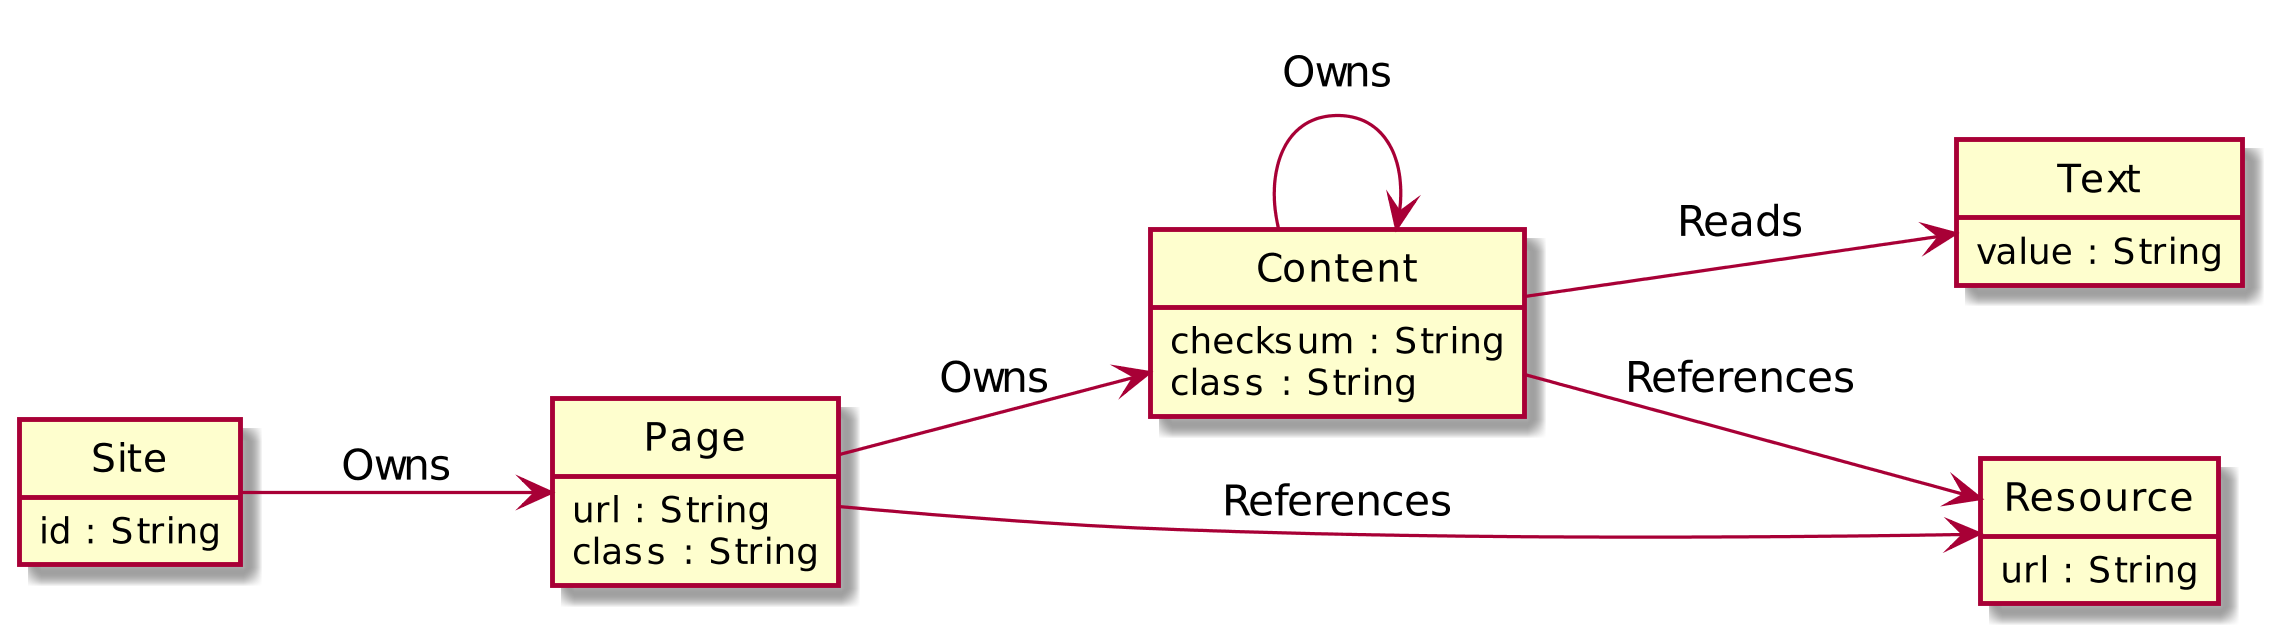
\includegraphics[scale=\imageScalingFactor]{../resources/db-data-model/nodes.png}
        \caption{Übersicht der Nodes und ihrer Beziehungen}
        \label{image:dbDataModelOverview}
    \end{figure}

    Entitäten, die als Node umgesetzt werden, sind Seiten, Content Features,
    der Text eines Content Features, referenzierte {\resources} und Sites.
    Diese erhalten die entsprechenden Labels Page, Content, Text, Reference und Site.
    Eine Seite kann als {\resource} existieren, bevor sie selbst klassifiziert wird.
    In diesem Fall erhält der Knoten zum Zeitpunkt der Klassifizierung zusätzlich auch das Label Page.

    Ein Seitenknoten speichert die \gls{url} der Seite, die auch als eindeutiger Identifier innerhalb der Datenbank dient,
    und die Klasse der Seite.

    Der Knoten einer {\resource} enthält lediglich ihre \gls{url}, die wiederum als eindeutiger Schlüssel dient.
    Wie später deutlich wird, kann er für alle Referenzen, die diese {\resource} als Ziel haben, genutzt werden.

    Knoten mit dem Label "`Content"' enthalten eine Prüfsumme über sich selbst, die innerhalb der Datenbank als Schlüssel Verwendung findet.
    Im späteren Verlauf geht Kapitel \ref{section:solutionDetailsClassificationStorageAPIUpdatePage} darauf ein,
    wieso diese Eigenschaft des Weiteren benötigt wird.
    Für skalare Content Features existiert exakt ein Knoten.
    Für CollectionFeatures existiert ein Knoten pro Element der Liste.

    Der Text eines Content Featuers wird in einem separaten Knoten gespeichert,
    der neben dieser Information nichts speichert und deshalb auch eindeutig über den Text identifiziert wird.
    Zwischen diesen beiden Knoten existiert deshalb eine Beziehung, die das Label Reads besitzt.
    Jeder Content Knoten ist maximal mit einem Textknoten verbunden.
    Der Grund für die Auslagerung ist, dass es viele Features geben kann, die den gleichen textuellen Inhalt besitzen.
    Die Intention ist diese Eigenschaft im Graphen explizit zu machen,
    sodass sie leicht für komplexere Analysen genutzt werden kann.
    Ein Anwendungsfall ist z. B. Informationen aus einer Datenbank,
    die auf verschiedene Seiten ausgegeben werden.
    Ein Text Knoten hat in diesem Fall viele eingehende Beziehungen,
    sodass leicht herausgefunden werden kann, auf welchen Seiten er enthalten ist.
    Eine explizite Beziehung ist dabei semantisch ausdrucksstärker und effizienter,
    als ein einfacher String-Vergleich, der über mit allen Knoten gemacht wird.
    Durch die Beziehung hat man die Info direkt.
    String-Vergleich ist auch dann nicht mehr sinnvoll, wenn man alle Knoten haben möchte,
    die sich einen Text teilen.
    Dann müsste man sehr viele Vergleiche durchführen.
    Durch die Beziehung ist es einfach nur alle Text Nodes, die mehrere einkommende Kanten haben.

    Zu guter Letzt speichern Site Knoten die ID der Site, wodurch der Knoten eindeutig identifiziert wird.
    Jede Seite kann mit beliebig vielen Page Knoten verbunden sein.
    Diese Beziehungen haben das Label Owns.

    Sowohl Seiten als auch Content Features können Content Features enthalten.
    Eine Seite ist zu jedem Content Feature mit einer eigenen Beziehung verbunden,
    die ebenfalls das Label Owns besitzt.
    Das gleiche gilt für Contents und ihre eigenen Content Features.
    Eine genauere Darstellung dieser Beziehung bietet Abbildung \ref{image:dbDataModelContentRelationship}.

    \begin{figure}
        \centering
        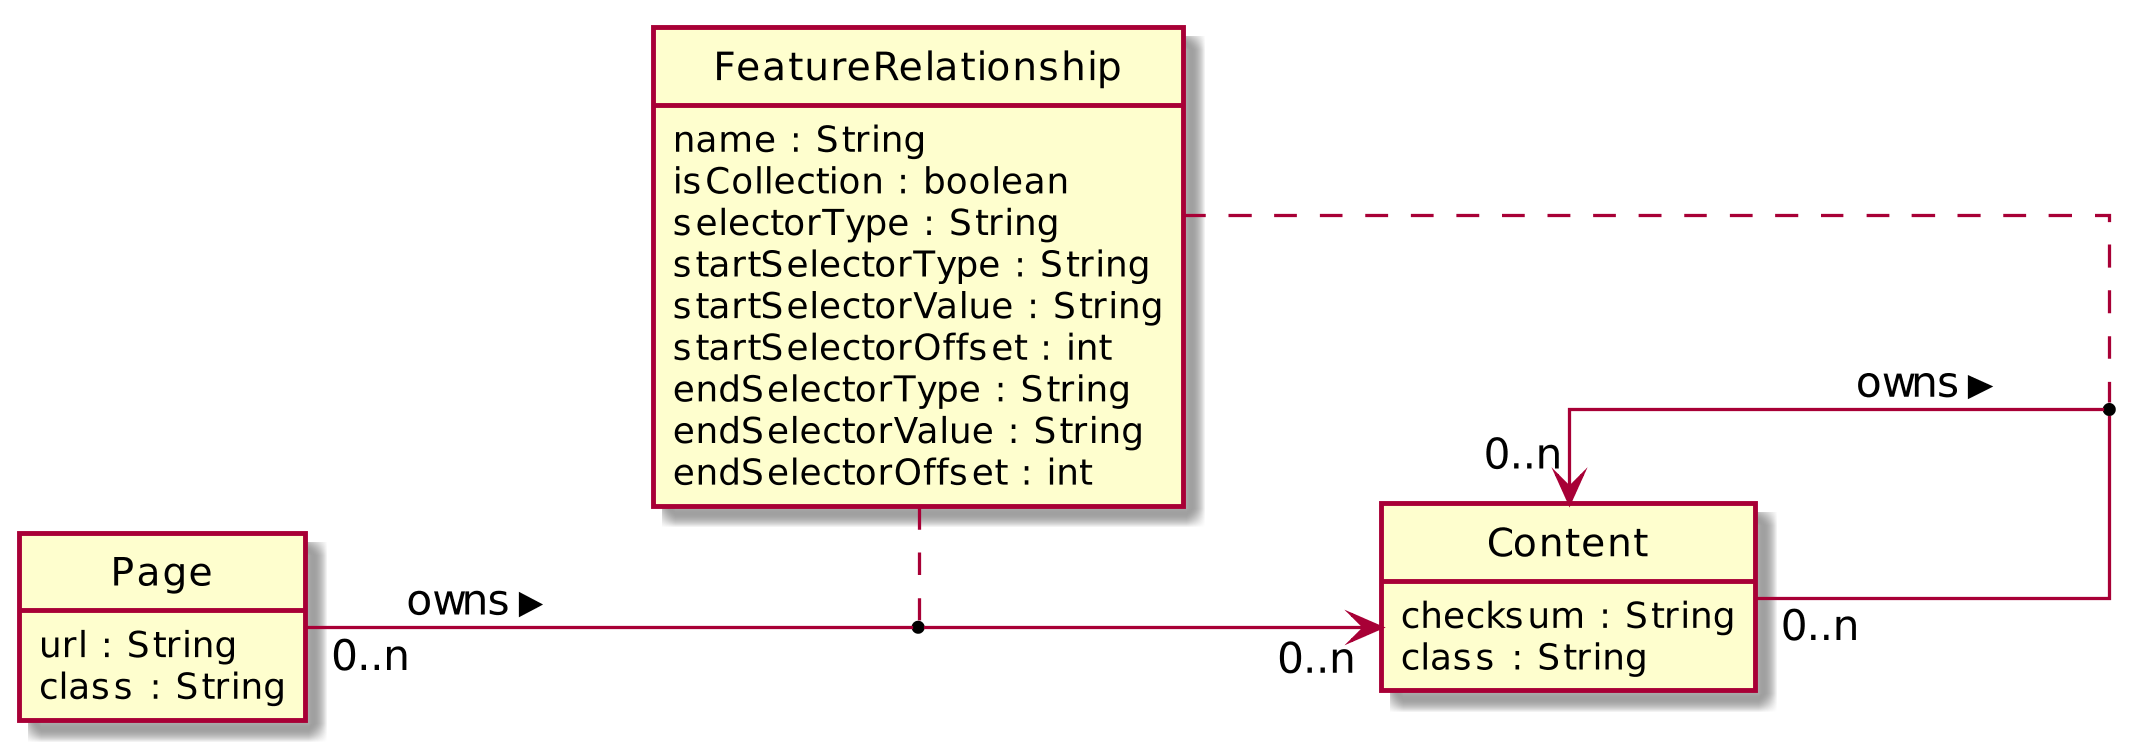
\includegraphics[scale=\imageScalingFactor]{../resources/db-data-model/content-relationship.png}
        \caption{Content Features}
        \label{image:dbDataModelContentRelationship}
    \end{figure}

    Eine Beziehung zwischen Page und Content bzw. Content und Content
    wird hier als FeatureRelationship bezeichnet.
    Eine solche Beziehung besitzt eine Reihe von Eigenschaften.
    Sie speichert den Namen des Features (name),
    ob es sich um ein Element eines CollectionFeatures handelt (isCollection)
    und den eindeutigen Selektor des Nodes, der zum Feature gehört
    (start-, endSelectorType; start-, endSelectorValue; start- endSelectorOffset, ).
    Bei Collection Features existieren viele ausgehende Kanten für ein Feature.
    Jede dieser Beziehungen speichert den gleichen Namen und hat isCollection auf true gesetzt.
    Es ist sinnvoll diese Informationen nicht im Content Knoten, sondern in der Beziehung zu speichern,
    um den Knoten besser wiederverwendbar zu machen.
    Details werden in Kapitel \ref{section:solutionDetailsClassificationStorageAPIUpdatePage} erklärt.

    Referenzen werden in der Datenbank durch eine Kombination aus
    {\resource} Knoten und Beziehungen zu diesen Knoten dargestellt.
    Page und Content Knoten können demanch eine ausgehende Beziehung zu einem
    {\resource} Knoten haben, die mit References markiert ist.
    Abbildung \ref{image:dbDataModelResourceRelationship} stellt diese Beziehung in den Fokus.

    \begin{figure}
        \centering
        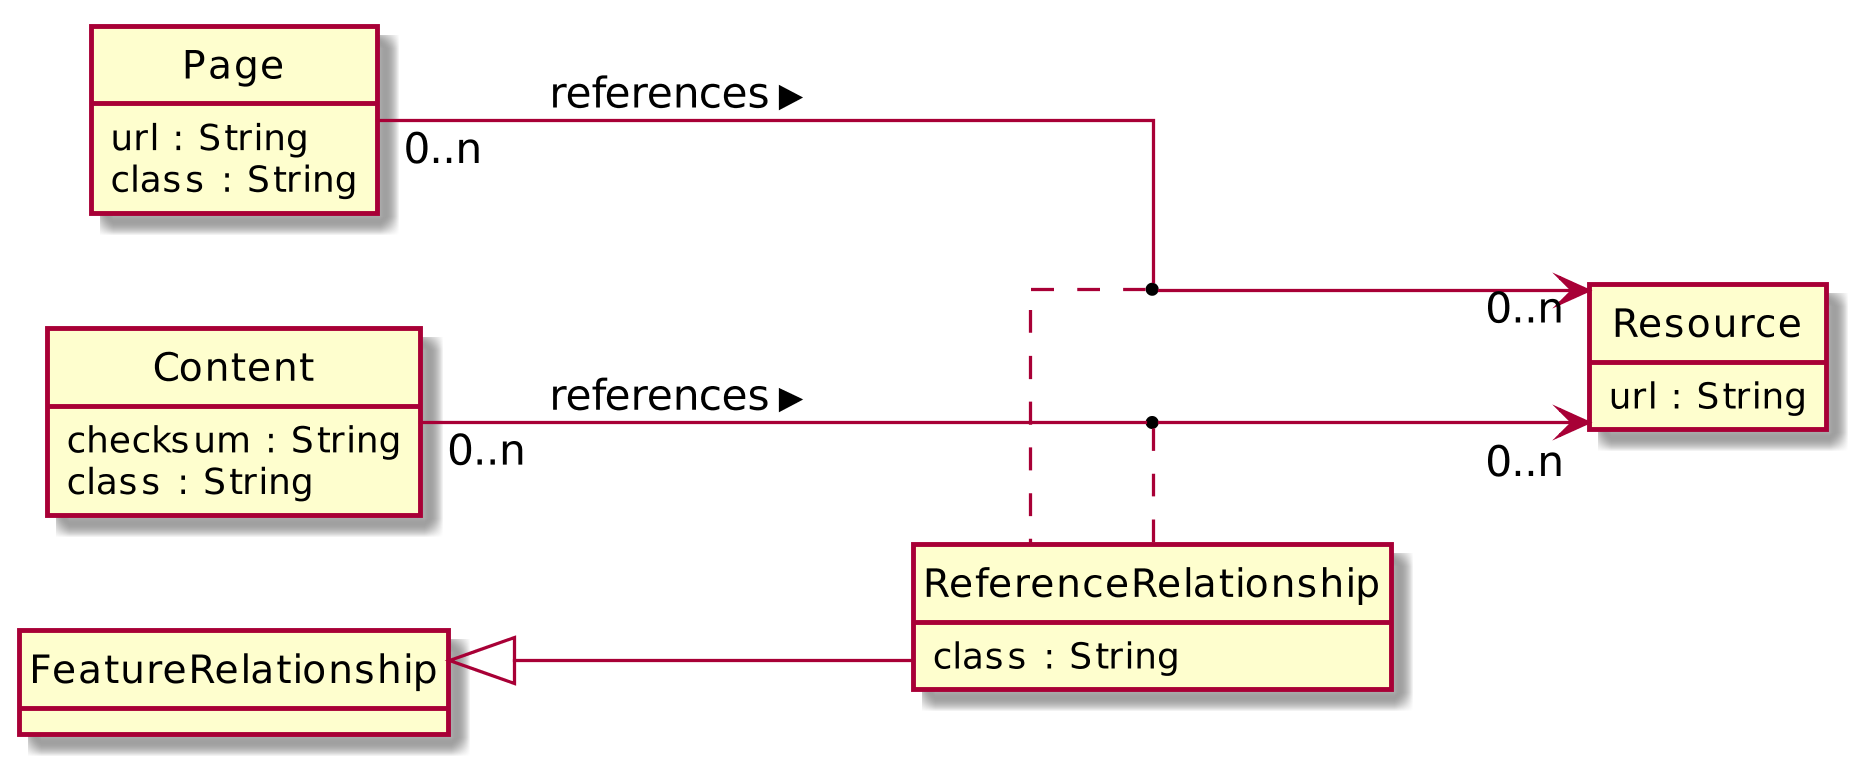
\includegraphics[scale=\imageScalingFactor]{../resources/db-data-model/resource-relationship.png}
        \caption{Reference Features}
        \label{image:dbDataModelResourceRelationship}
    \end{figure}

    Wie zu sehen ist, handelt es sich bei einer ReferenceRelationship ebenfalls
    um eine FeatureRelationship, weshalb sie ebenfalls die oben beschriebenen Informationen speichert.
    Zusätzlich enthält sie aber auch die Klasse der Referenz.
    Diese kann nicht im {\resource} Knoten gespeichert werden,
    da der Knoten für viele Referenzen dienen kann und die Klasse nicht überall identisch sein muss.
    \subsection{Beispiel einer Klassifikation}
    \label{section:solutionDetailPersistenceDataModelExample}
    Um das eben beschriebene Datenmodell greifbarer zu machen,
    präsentiert dieses Kapitel, wie eine konkrete Klassifikation als
    Graph im {\classificationStorage} gespeichert wird.
    Spätere Erklärungen nehmen auf dieses Beispiel ebenfalls Bezug.
    Eine Übersicht der Knoten des Beispielgraphen wurde aus Gründen
    der Übersichtlichkeit auf die Abbildungen \ref{image:dbDataModelExampleOverviewPart1}
    und \ref{image:dbDataModelExampleOverviewPart2} verteilt.
    Sie sind über den \texttt{Content}-Knoten \texttt{c5} verbunden
    und verzichten zunächst auf die ausführliche Darstellung der Eigenschaften der Beziehungen.

    \begin{figure}[htb]
        \centering
        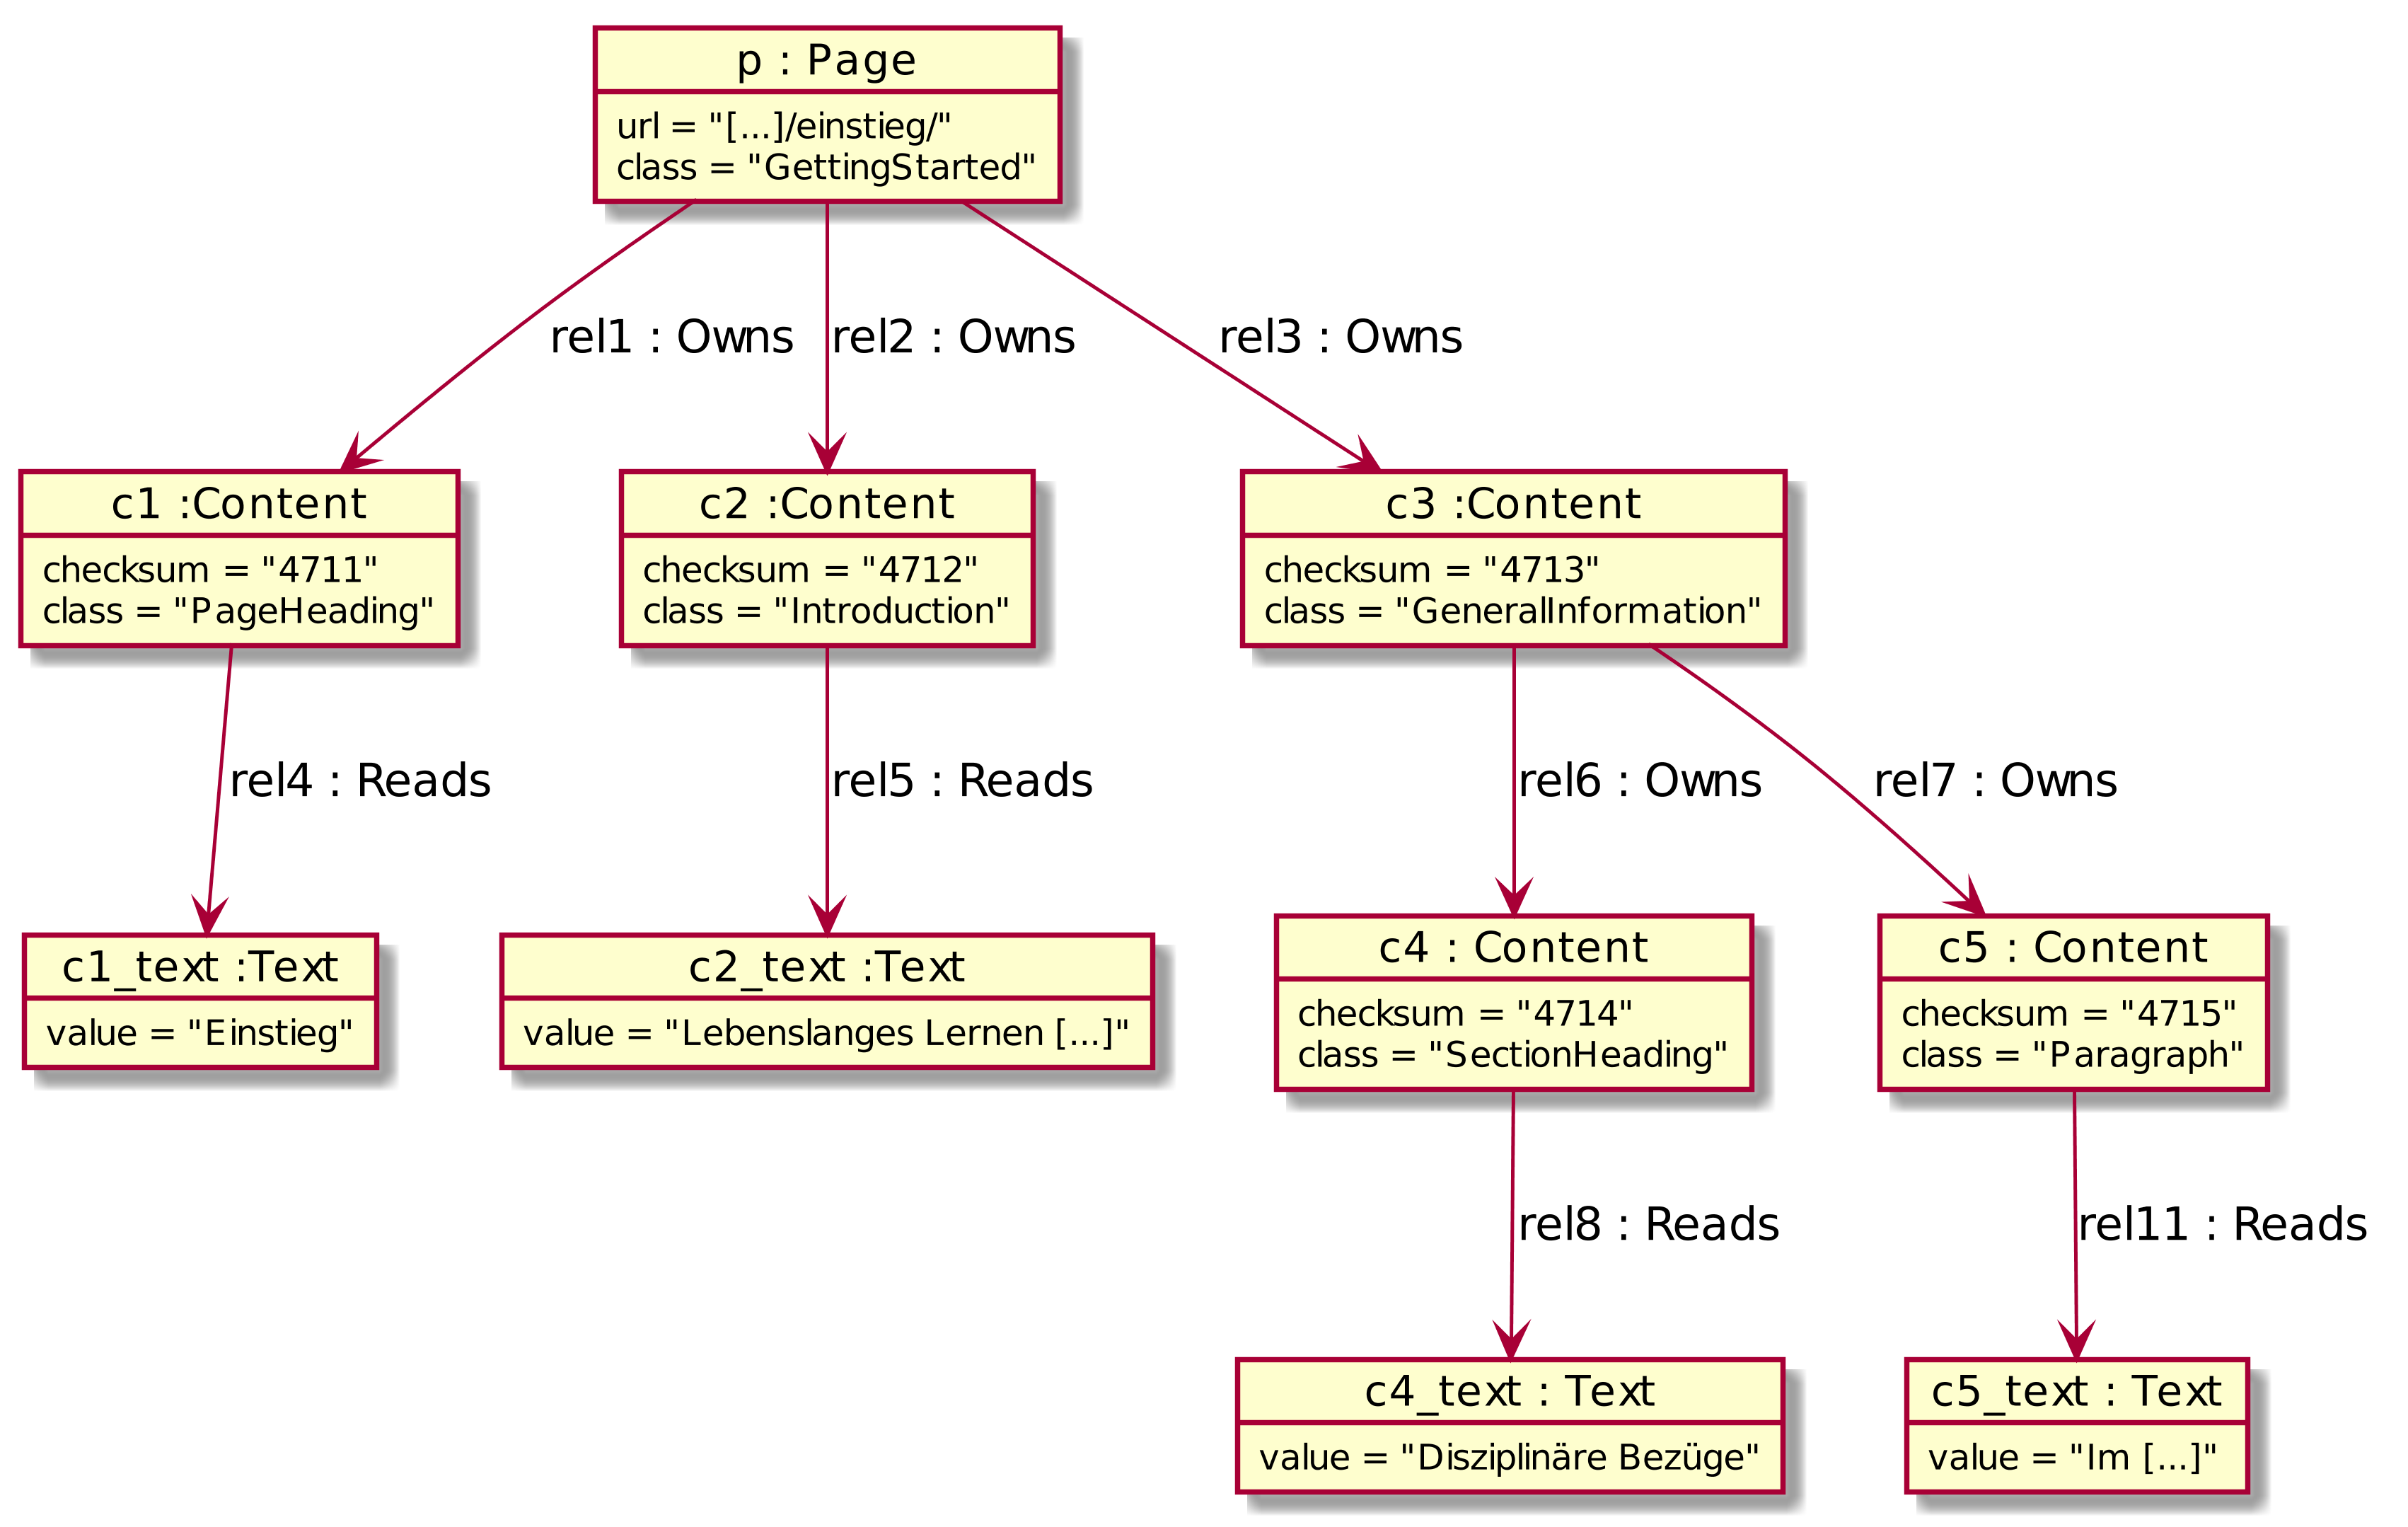
\includegraphics[scale=\imageScalingFactor]{../resources/db-data-model/example/example_part1.png}
        \caption{Ein Beispiel einer Klassifikation im {\classificationStorage} (1)}
        \label{image:dbDataModelExampleOverviewPart1}
    \end{figure}

    Die betroffene Webseite wurde als "`GettingStarted"' klassifiziert und besitzt drei skalare {\contentFeature}s,
    für die \texttt{Content}-Knoten existieren.
    Der \texttt{Page}-Knoten ist mit ihnen über \texttt{Owns}-Beziehungen verbunden.
    Die Inhalte \texttt{c1} und \texttt{c2} beinhalten Text und sind deshalb mit entsprechenden \texttt{Text}-Knoten verbunden.
    Der Knoten \texttt{c3} hat hingegen zwei {\childFeature}s (\texttt{c4} und \texttt{c5}), die seinen Text feingranular speichern
    und deshalb ihrerseits mit \texttt{Text}-Knoten verbunden sind.
    In Abbildung \ref{image:dbDataModelExampleOverviewPart2} ist zu sehen,
    dass \texttt{c5} neben seinem Text auch zwei {\resources} referenziert,
    die durch entsprechende \texttt{Resource}-Knoten dargestellt werden.

    \begin{figure}[htb]
        \centering
        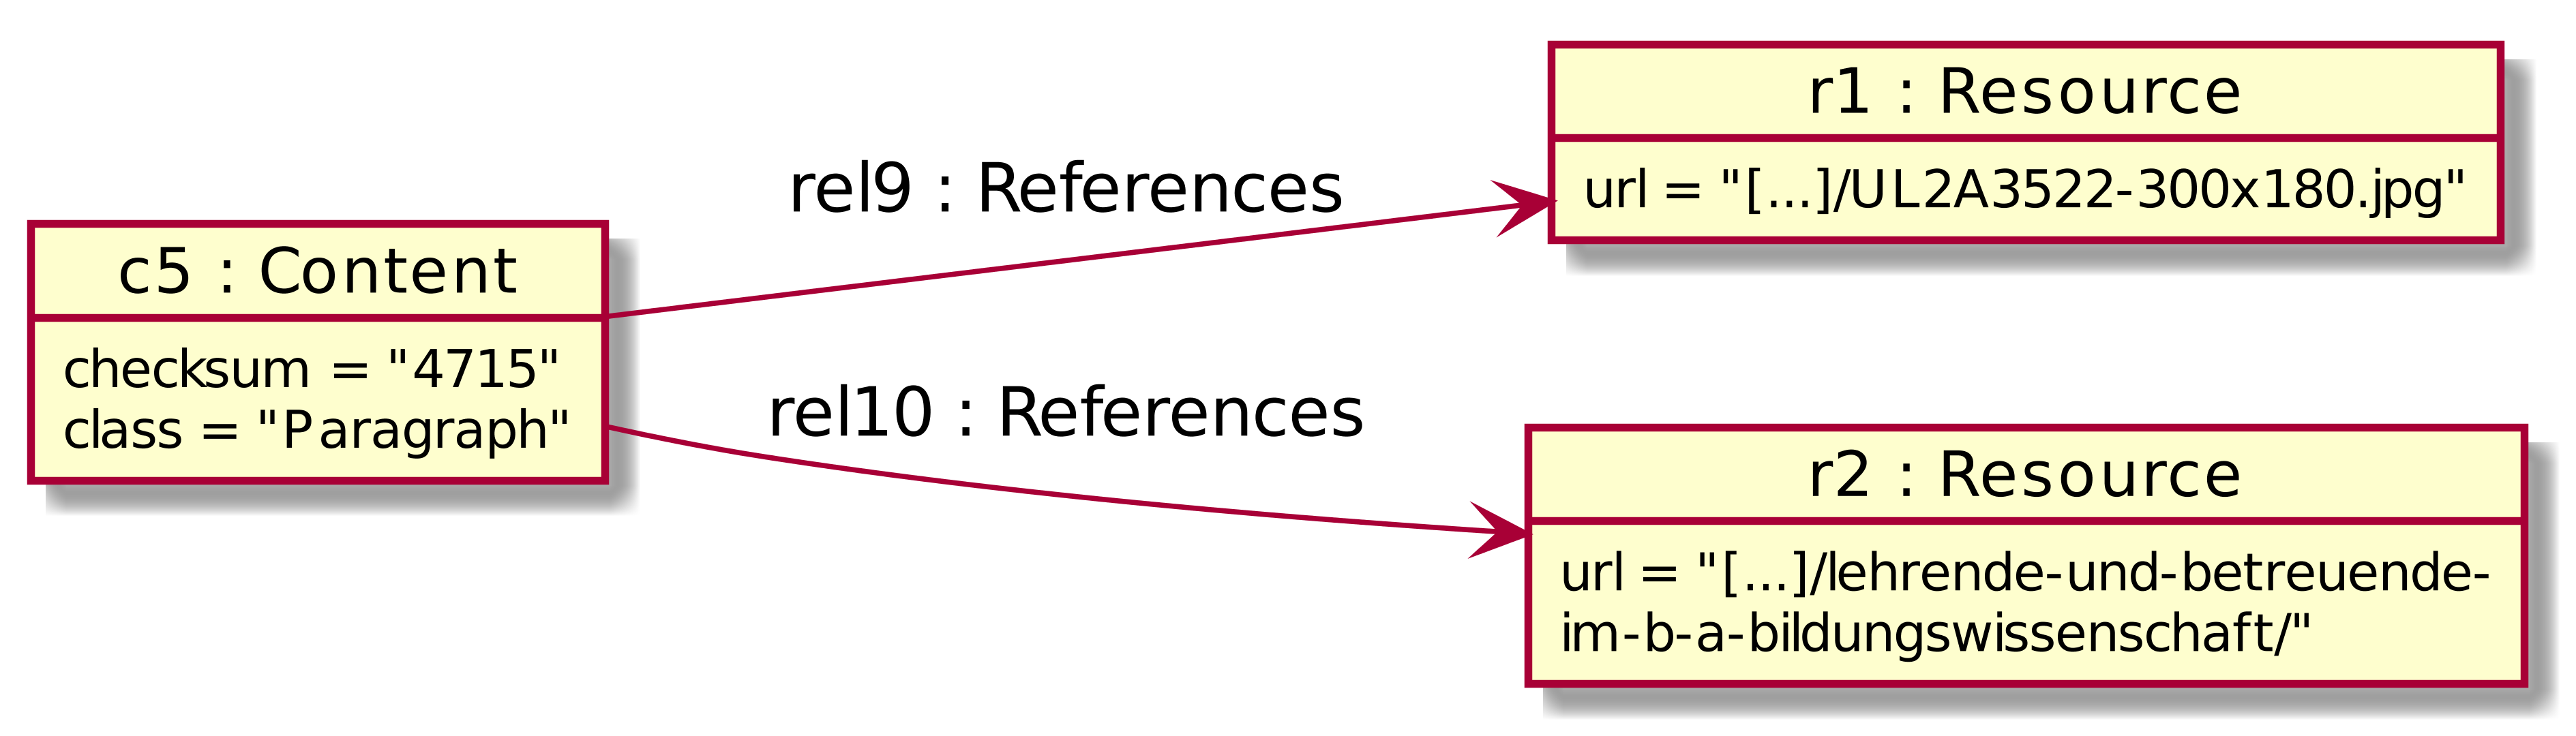
\includegraphics[scale=\imageScalingFactor]{../resources/db-data-model/example/example_part2.png}
        \caption{Ein Beispiel einer Klassifikation im {\classificationStorage} (2)}
        \label{image:dbDataModelExampleOverviewPart2}
    \end{figure}

    Bei diesen Referenzen handelt es sich um ein {\collectionFeature},
    was aus Abbildung \ref{image:dbDataModelExampleRel10} hervorgeht,
    die eine Beziehung zu einem \texttt{Resource}-Knoten detailliert darstellt.

    \begin{figure}[htb]
        \centering
        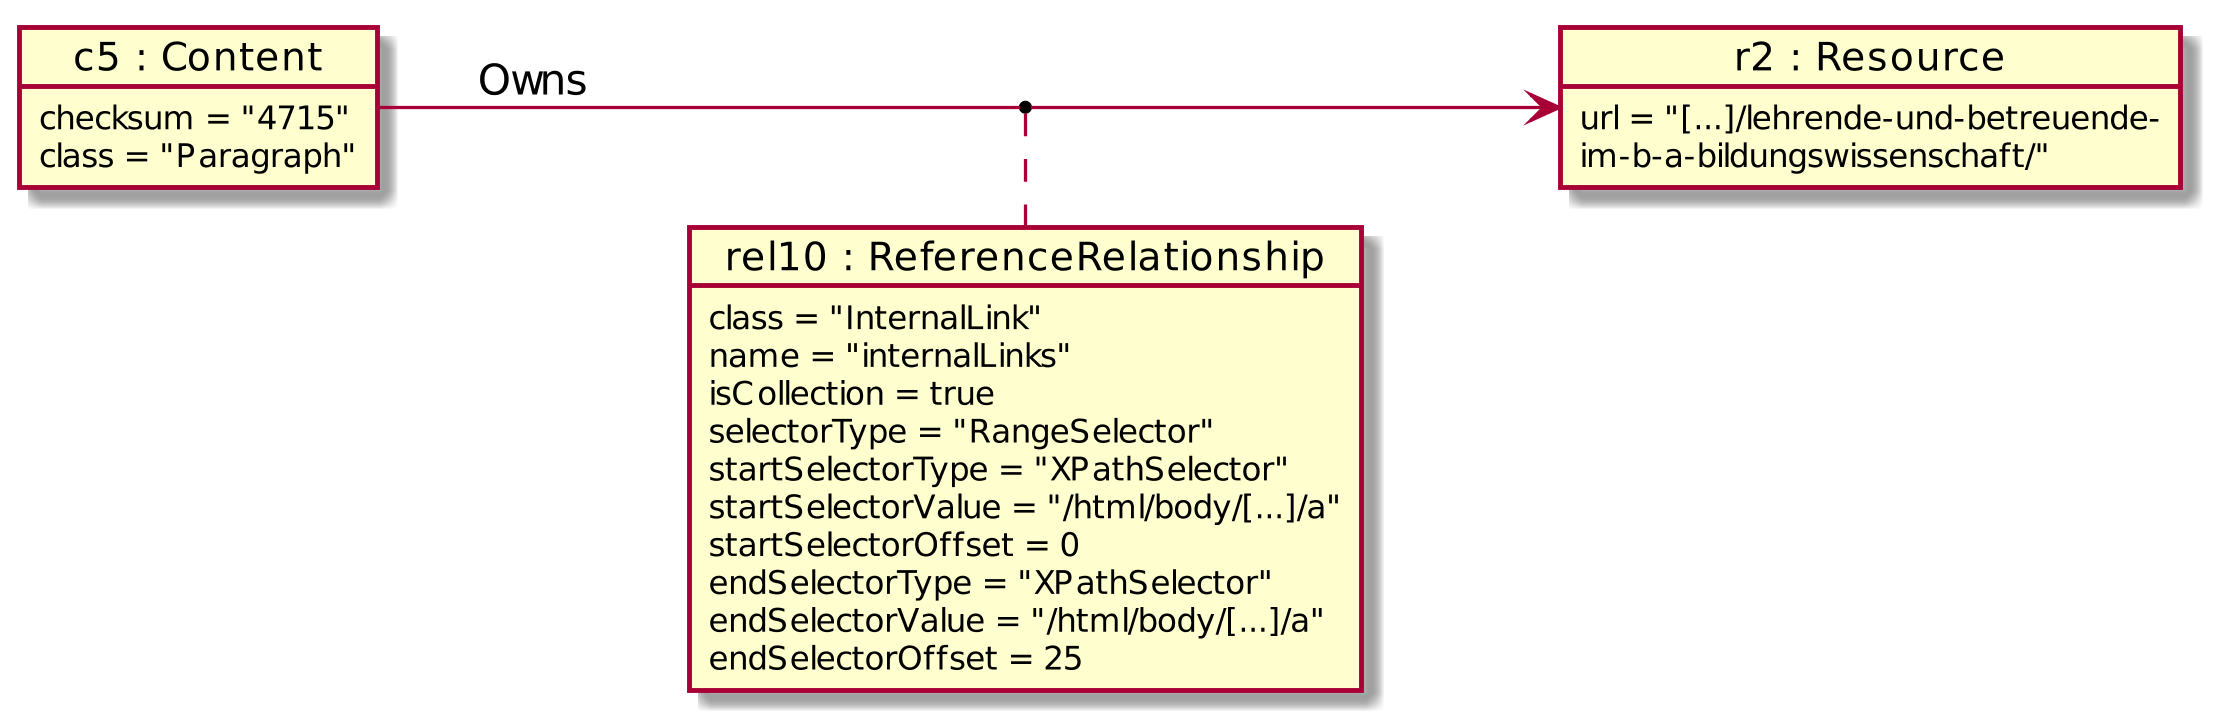
\includegraphics[scale=\imageScalingFactor]{../resources/db-data-model/example/c5-r2.png}
        \caption{Ein Beispiel einer Beziehung zu einem {\resource}-Knoten}
        \label{image:dbDataModelExampleRel10}
    \end{figure}

    Die Eigenschaft \texttt{isCollection} besitzt nämlich den Wert \texttt{true}.
    Des Weiteren wird hier deutlich, wie die Informationen des eindeutigen Selektors gespeichert werden.
    Dem Datenmodell folgend ist eine konkrete Beziehung zu einem \texttt{Content}-Knoten
    sehr ähnlich aufgebaut. Wie in Abbildung \ref{image:dbDataModelExampleRel1} zu sehen,
    verzichtet sie lediglich auf die Speicherung der Klasse.

    \begin{figure}[htb]
        \centering
        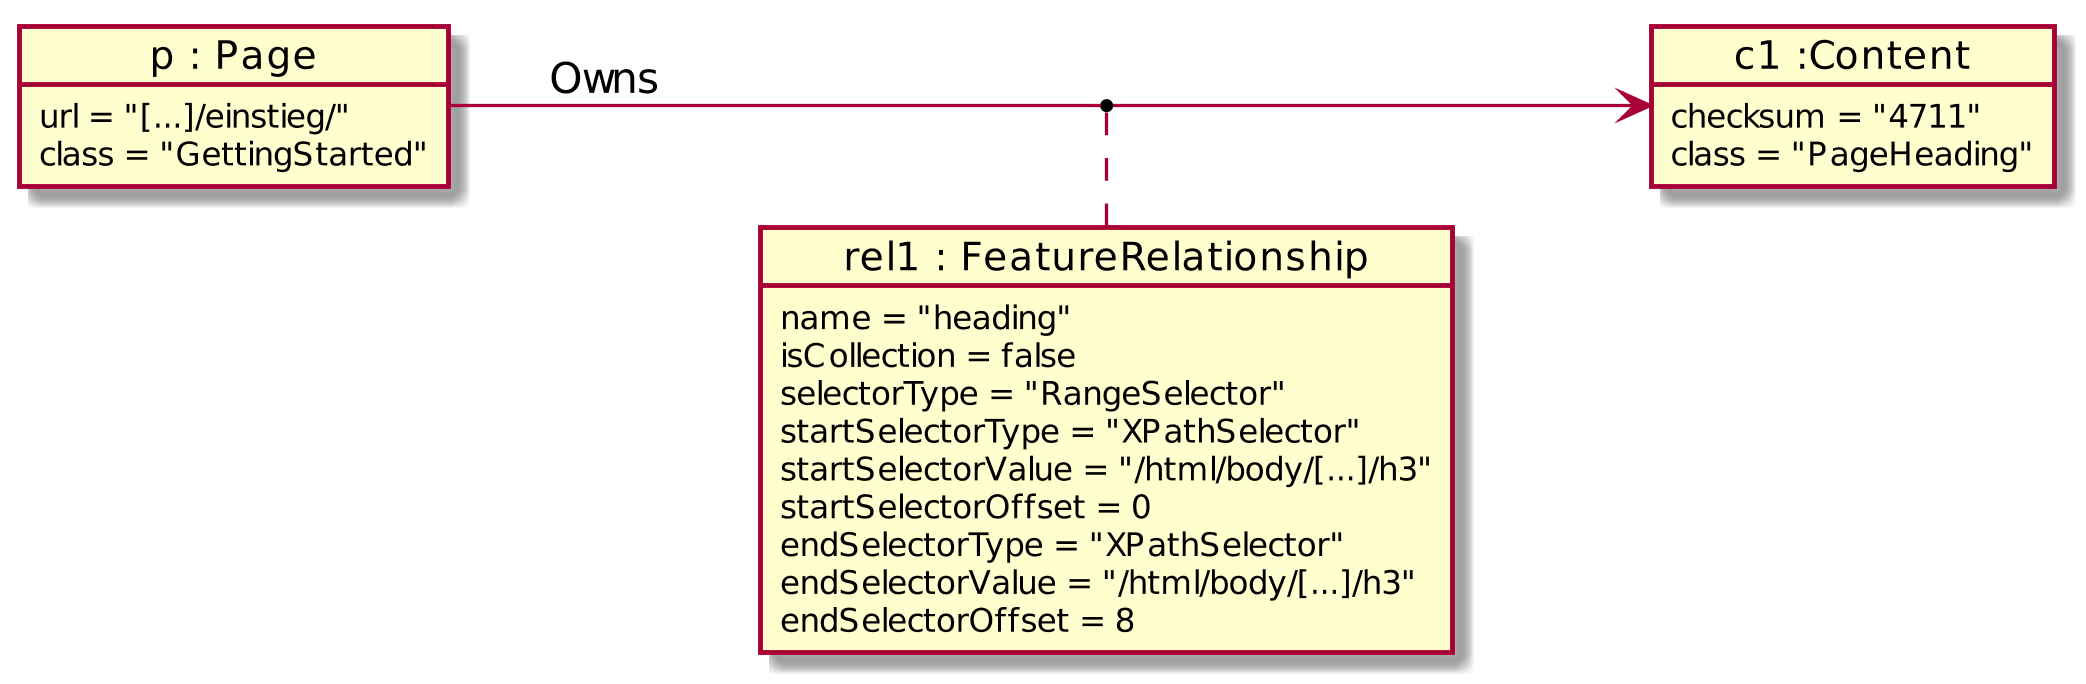
\includegraphics[scale=\imageScalingFactor]{../resources/db-data-model/example/p-c1.png}
        \caption{Ein Beispiel einer Beziehung zu einem Content-Knoten}
        \label{image:dbDataModelExampleRel1}
    \end{figure}

    \subsection{Eignung einer Graphdatenbank}
    Die Nutzung einer Graphdatenbank für das \gls{wccs} hat mehrere Beweggründe.
    Dazu zählen die einfache, natürliche und schemalose Datenmodellierung
    und die Möglichkeit Beziehungen sehr einfach auszuwerten.
    Die Wiederverwendung von Knoten für mehrere Klassifikationen
    bietet außerdem die Möglichkeit, weiterführende Analysen auf den
    klassifizierten Inhalten durchzuführen.
    Dieses Kapitel bewertet die tatsächliche Eignung einer Graphdatenbank,
    des verwendeten Datenmodells sowie des Algorithmus
    zum Schreiben von Klassifikationen, der das Teilen von Knoten ermöglicht.

    \paragraph*{Referenzen zwischen Webseiten}
    Das zweite Fallbeispiel hat gezeigt,
    wie Referenzen zwischen Webseiten auf sehr einfache Art und Weise
    Reihenfolgen und Navigationspfade (der Nachrichtenseiten) explizit machen.
    Eine Auswertung ist trivial, da lediglich ein- und ausgehenden Kanten gefolgt werden muss.
    Andere Datenbankmodelle hätten komplexere Konstrukte
    zur Speicherung und zur Auswertung erfordert.

    \paragraph*{Wiederverwendung von Text- und Resource-Knoten}
    Betrachtet man Tabelle \ref{table:findingsTeachersFiguresNodesByLabel}, wird deutlich,
    dass \texttt{Text}- und \texttt{Resource}-Knoten verhältnismäßig am meisten von der
    Wiederverwendbarkeit Gebrauch machen.
    Das ist nicht verwunderlich, da sie jeweils genau einen Wert speichern,
    der sie identifiziert.
    Gleichzeitig besitzen sie keine ausgehenden Kanten,
    die seitenspezifische Informationen enthalten.
    Wie Tabelle \ref{table:findingsTeachersFiguresSharedNodes} belegt,
    steigt ihre Wiederverwendung bei mehreren Klassifikationen in einer Datenbank,
    was eine logische Konsequenz der größeren Datenmenge ist.
    Für \texttt{Resource}-Knoten ist das aber nicht sofort ersichtlich, da
    die Summe der mehrfach verwendeten \texttt{Resource}-Knoten von Lehrgebieten
    im Falle einzelner Datenbanken höher ist, als im Fall einer gemeinsamen Datenbank (36 vs. 30).
    Gleichzeitig ist die Zahl der geteilten \texttt{SubjectArea}-Knoten aber höher,
    die jeder einen \texttt{Resource}-Knoten eines Lehrgebietes referenzieren.
    Es wird also ein größerer Teil des Graphen wiederverwendet.
    Außerdem enthielten die einzelnen Datenbanken identische \texttt{Resource}-Knoten,
    die in der gemeinsamen natürlich zusammengefasst werden konnten.

    \paragraph*{Entbehrlichkeit von Text-Knoten}
    Innerhalb einer Datenbank macht es aus semantischen Gründen keinen Sinn
    \texttt{Resource}-Knoten zu duplizieren,
    da sie eine Entität der Domäne darstellen.
    {\resources} existieren genau ein mal, was die Datenbank widerspiegeln sollte
    und außerdem die Möglichkeiten eines Graphen besser ausschöpft.
    Nicht so eindeutig ist dies allerdings bei \texttt{Text}-Knoten.
    Aus Tabelle \ref{table:findingsTeachersFiguresSharedNodes} geht hervor,
    dass im ersten Fallbeispiel niemals ein \texttt{Text}-Knoten geteilt wurde.
    Stattdessen konnte immer der zugehörige \texttt{Content}-Knoten geteilt werden.
    Deshalb ist die Zahl beider Knotentypen gesunken und die der geteilten
    \texttt{Content}-Knoten dafür gestiegen.
    Tabelle \ref{table:findingsNewsFiguresSharedNodes}
    zeigt eine andere Situation beim zweiten Fallbeispiel.
    Dort werden zwei \texttt{Text}-Knoten geteilt,
    weil es mehrere Nachrichten mit derselben Überschrift gibt.
    Sie referenzieren aber unterschiedliche Detailseiten,
    weshalb die Nachrichten unterschiedliche \texttt{Content}-Knoten besitzen.
    Der tatsächliche Nutzen der \texttt{Text}-Knoten ist in beiden Beispielen trotzdem sehr gering.
    Der textuelle Wert eines {\contentFeature}s ist deshalb im \texttt{Content}-Knoten selbst besser aufgehoben.
    Für die Schnittstellen des \glspl{wccs} ändert sich durch eine entsprechende Anpassung nichts,
    allerdings vereinfacht sich das Datenmodell der Datenbank sowie
    die generierten Datenbankanweisungen.

    \paragraph*{Hierarchieebene wiederverwendeter Teilgraphen}
    Bezüglich der Wiederverwendung von Teilgraphen ist außerdem ersichtlich,
    dass sie häufig erst auf einer tiefen Ebene des Graphen stattfindet.
    \texttt{Content}-Knoten der Klasse \texttt{SubjectAreaName} werden bspw.
    sehr viel häufiger von mehreren Klassifikationen verwendet als solche der
    Klasse \texttt{Teacher}.
    Betrachtet man die klassifizierten Webseiten,
    ist eine entgegengesetzte Erwartung gerechtfertigt.
    Der Kopfbereich wiederholt sich z. B. auf allen Seiten
    und mehrere Mitarbeiter werden auf unterschiedlichen Webseiten identisch aufgeführt.
    Trotzdem wird bei solchen Mitarbeitern und dem Kopfbereich
    nicht der \texttt{Teacher}- bzw. \texttt{Header}-Knoten geteilt,
    sondern nur ihre Unterknoten.
    Dafür gibt es zwei Gründe.
    Zum einen müssen Features inklusive ihrer {\childFeature}s inhaltlich
    exakt übereinstimmen, damit ihr \texttt{Content}-Knoten mehrfach verwendet werden kann.
    Die kleinste Abweichung macht dies unmöglich,
    da die Inhalte sich letztendlich unterscheiden und nur Teilaspekte übereinstimmen.
    Das muss die Datenbank widerspiegeln.
    Im Falle des Kopfbereiches im ersten Beispiel ist die \gls{url} des Logos
    auf jeder Seite unterschiedlich.
    Das ist im zweiten Beispiel nicht der Fall,
    da alle Seiten zu einem Portal in {\wordpress} gehören
    und deshalb das gleiche Bild referenzieren.
    Deshalb existiert in der Datenbank nur ein \texttt{Header}-Knoten,
    den alle Klassifikationen referenzieren.
    Die zweite Ursache sind unterschiedliche Positionen identischer Inhalte
    auf verschiedenen Webseiten.
    Diese Positionen werden in Form des eindeutigen Selektors in der eingehenden
    Kante eines \texttt{Content}-Knotens gespeichert\footnote{vgl. Kapitel \ref{section:solutionDetailsPersistenceDataModel}}.
    Diese Knoten sind prinzipiell also unabhängig von der konkreten Position
    von mehreren Klassifikationen gleichzeitig nutzbar.
    Dies ändert sich allerdings, sobald ein Inhalt {\childFeature}s besitzt.
    Die ausgehenden Kanten zu diesen Features speichern ihre \textit{absoluten} Selektoren.
    Befindet sich ein Mitarbeiter auf zwei Seiten also nicht an exakt der gleichen Position,
    sind die Selektoren seines Namens, seines Lehrgebietes etc. unterschiedlich.
    Der \texttt{Teacher}-Knoten kann dann nicht von beiden Klassifikationen referenziert
    werden.
    
    \paragraph*{Semantischer Inhalt und physische Struktur einer Webseite}
    Genau betrachtet spiegelt die Datenbank lediglich die Struktur der Webseiten exakt wider.
    Trotzdem lässt sich argumentieren, dass es fachlich konsistenter wäre,
    wenn die \texttt{Teacher}-Knoten im oben beschriebenen Fall geteilt werden würden.
    Ein Beispiel verdeutlicht das:
    Schon jetzt lässt sich die Frage beantworten,
    welche Mitarbeiter in einem gewissen Lehrgebiet arbeiten.
    Dazu muss lediglich den eingehenden Kanten eines
    \texttt{SubjectAreaName}-Knotens über alle \texttt{SubjectArea}-Knoten
    bis zu \texttt{Teacher}-Knoten gefolgt werden.
    Aus fachlicher Sicht ist es aber inkonsistent,
    dass man diese Suche nicht beim \texttt{SubjectArea}-Knoten
    starten kann, weil mehrere dieser Knoten denselben
    \texttt{SubjectAreaName}-Knoten verwenden.
    Aus fachlicher Sicht existieren laut Datenbank also mehrere Lehrgebiete,
    die denselben Namen tragen.
    Hier wird ein Konflikt zwischen dem akkuraten Widerspiegeln der Strukturen der Webseiten
    und dem semantischen Inhalt deutlich.

    \paragraph*{Alternativen}
    Ein erster Schritt zur Auflösung dieses Konfliktes ist, anstatt absolute Selektoren
    lediglich zum {\parentFeature} relative Selektoren in den Kanten zu speichern.
    Allerdings hilft dies nicht, wenn die HTML-Struktur sich unterscheidet,
    weil dann auch die relative Position eines Elementes anders ist.
    Außerdem hätte dies zur Folge, dass zur Ermittlung der eindeutigen Position
    eines Features, der gesamte Vaterpfad bis zur Seite abgelaufen werden muss.
    Eine weitere Alternative zum aktuellen Vorgehen,
    die auch diesen Nachteil umgeht,
    ist die Speicherung der absoluten Selektoren in Kanten,
    die vom \texttt{Page}-Knoten direkt zu \texttt{Content}-Knoten führen.
    Die Teilbarkeit von Content Knoten hinge dann nur noch von den Inhalten und ihrer Klasse ab,
    da die Position komplett unabhängig gespeichert wird.

    \paragraph*{Änderung von Klassifikationen}
    Durch den entwickelten Algorithmus zum Schreiben von Klassifikationen
    wurde das Teilen von Knoten ermöglicht.
    Eine nachteilige Folge ist allerdings,
    dass Änderungen immer über diesen Algorithmus eingearbeitet werden müssen,
    weil sonst Inkonsistenzen riskiert werden.
    Falls die Analysemöglichkeiten keine praktische Relevanz haben,
    ist deshalb ein anderer Datenbanktyp, wie zum Beispiel ein einfacher Document Store,
    in Betracht zu ziehen.

    Insgesamt scheint eine Graphdatenbank trotz der genannten Herausforderungen geeignet
    für den Anwendungsfall des \glspl{wccs}.

